\section{The Greenhouse Effect}
\label{greenhouse_effect}

Up to now we have considered a very crude model in which the Earth is a black body with no atmosphere, and its energy 
balance is ruled by the incoming solar radiation and the outgoing long wave radiation (\gls{LW}). We have seen
that such a model gave us a temperature that is significantly below the one that we observe. This is due to the 
\textbf{greenhouse effect}.

\subsection{Emissivity, Absorptivity and Transmissivity}
We can now come up with a more nuanced model of the Earth's energy balance. First we need to consider that materials are
not perfect emitters, so we definte the \textbf{\gls{emissivity}} $\epsilon_\lambda$ of 
a material as the ratio of the irradinace emitted by the material to the irradiance emitted by a black body at the same
temperature. Notice that the \gls{emissivity} is a function of wavelength. 
$$
\epsilon_\lambda = \frac{I_{\text{material}}}{I_{\text{black body}}}
$$

By definition, a black body has an \gls{emissivity} of $\epsilon_{BB} = 1$ so it follows that 
$I_{\text{material}} = \epsilon_\lambda \sigma T^4$. A material that emits like a \textbf{grey body} is one that has a 
constant \gls{emissivity} across all wavelengths. \\

\noindent We can also define the \textbf{\gls{absorptivity}} $a_\lambda$ of a
material as the ratio of the irradiance actually absorbed by the material to the irradiance incident on it. This is also
a function of wavelength and is always a number between 0 and 1, meaning actual materials absorb less than a black body.
It follows that, by definition, the \gls{absorptivity} of a black body is 
$a_{BB} = 1 = \epsilon_\lambda$ and in general (for systems in local thermodynamical equillibrium, as per Kirchoff's Law)
$a_\lambda = \epsilon_\lambda$.\\

\noindent Finally, the more absorbing a material is, the less radiation it will transmit. We define the 
\textbf{\gls{transmissivity}} $t_\lambda$ of a material as $1 - a_\lambda = 1 - \epsilon_\lambda$.
 This is also a function of wavelength and is always a number between 0 and 1. This relationship only
holds in the absence of scattering, a reasonable assumption for clear-sky \gls{LW} radiation.

\subsection{Optical Depth}
\label{sec:opticaldepth}

We can also write transmissivity in terms of the \hyperlink{glo:opticaldepth}{optical depth} $\tau_\lambda$ of a
material as follows:
$$
t_\lambda = e^{-\tau_\lambda} \quad \implies \quad \tau_\lambda = \int_0^\infty k_{a \lambda} \rho_{a} dz
$$
where \hypertarget{absorption_coefficient}{$k_{a \lambda}$} is the \textbf{absorption coefficient} of the material, 
$\rho_a$ is the density of the material across the atmosphere $dz$. 

The optical depth is dimensionless: it the atmosphere
has a $\tau$ of 1 it means that the amount of radiation transmitted through it from the surface to the \gls{TOA}
is reduced by a factor of $1/e$. Increasing the amount of absorbing material in the atmosphere will increase $\tau_\lambda$
and therefore reduce $t_\lambda$.

\subsection{Deffinition of, and a Simple Model of the Greenhouse Effect}
\label{sec:greenhouse_definition}
We will define the \textbf{greenhouse effect} ($G$) as the amount of \gls{LW} radiation emitted by the Earth's
surface that is trapped within the Earth's atmosphere. We can see how the atmosphere interacts with \gls{LW}
and \gls{SW} radiation in figure \ref{fig:transmitted_radiation}.

\begin{figure}[h]
    \centering
    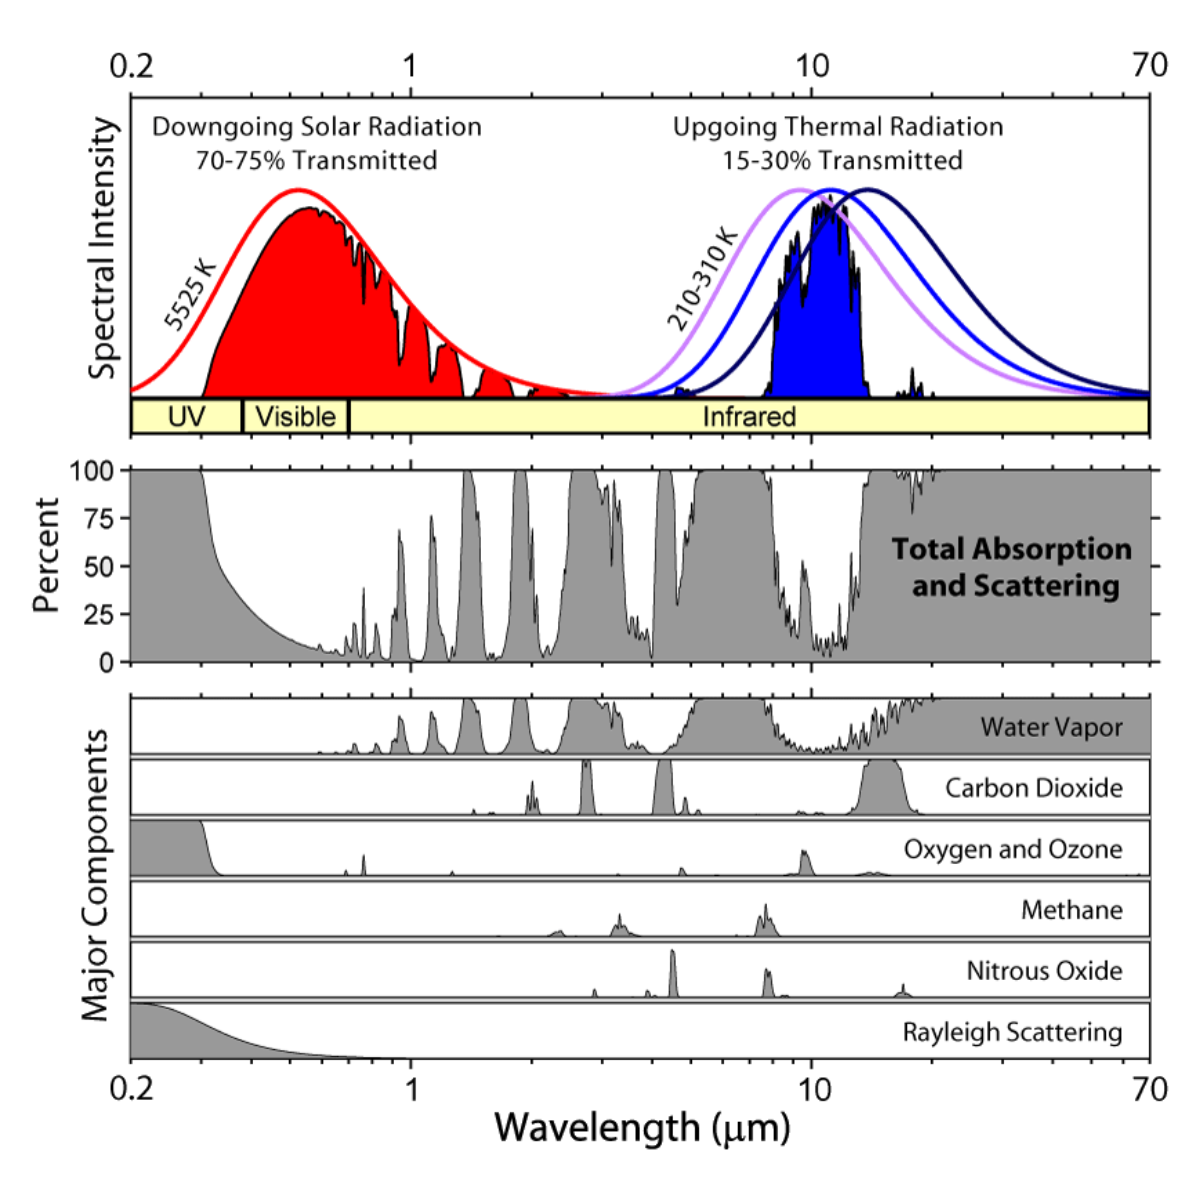
\includegraphics[width=0.65\textwidth]{figures/transmitted_radiation.png}
    \caption{Radiation Transmitted by the Atmosphere.}
    \label{fig:transmitted_radiation}
\end{figure}

As per figure \ref{fig:transmitted_radiation}, the atmosphere is much more transparent to \gls{SW} radiation than
it is to \gls{LW} radiation. Water vapour is the main absorber of \gls{LW} radiation followed by
carbon dioxide and some other gases. If we assume the Earth's surface has a temperature $T_s$ and it emmits as a black
body, then we can define $G$ as:
$$
\boxed{
    G = \sigma T_s^4 - \text{\gls{OLR}}
}
$$
where \gls{OLR} is the \textbf{outgoing long wave radiation} at the \gls{TOA}, i.e. the sum total
of radiation that escapes Earth into space.\\

\noindent Let us introduce a simple model of the greenhouse effect. We will have a few (important) assumptions:
\begin{itemize}
    \item The atmosphere is completely transparent to \textbf{solar radiation} (\gls{SW}).
    \item We have blackbody emissioin from the surface at temperature $T_s$.
    \item The atmosphere is a single layer grey-body with \gls{emissivity} $\epsilon_a$ and
    temperature $T_a$ emitting in the upward and downward directions equally.
    \item There is \textbf{radiative equillibrium} at the surface, in the atmosphere and at the \gls{TOA}.
\end{itemize}

In this case, by energy conservation we can write the following for the \textbf{top of the atmosphere}:
\begin{equation}
    \begin{aligned}
    &\begin{tabular}{c}
    Incoming \\ \gls{SW} from the Sun
    \end{tabular}
    & = 
    &\begin{tabular}{c}
    \gls{LW} emitted \\ by the atmosphere
    \end{tabular}
    & + 
    &\begin{tabular}{c}
    Transmitted \\ \gls{LW} from the surface
    \end{tabular} \\
    &\makebox[3.7cm]{$\displaystyle\frac{(1 - \alpha_p)\ \text{\gls{TSI}}}{4}$} & = &\makebox[4cm]{$\epsilon_a 
    \sigma T_a^4$} & + &\makebox[4cm]{$(1 - \epsilon_a) \sigma T_s^4$}
    \end{aligned}
    \nonumber
\end{equation}
\textbf{within the atmosphere} we can write:
\begin{equation}
    \begin{aligned}
    &\begin{tabular}{c}
    \gls{LW} emitted by the \\ surface absorbed by atmos
    \end{tabular}
    & = 
    &\begin{tabular}{c}
    \gls{LW} emitted by the \\ atmosphere up and down
    \end{tabular}\\
    &\makebox[5.5cm]{$\displaystyle\epsilon_a \sigma T_s^4$} & = &\makebox[5cm]{$2 \epsilon_a \sigma T_a^4$}
    \end{aligned}
    \nonumber
\end{equation}
finally, \textbf{at the surface} we can write:
\begin{equation}
    \begin{aligned}
    &\begin{tabular}{c}
    \gls{LW} emitted \\ by the surface    
    \end{tabular}
    & = 
    &\begin{tabular}{c}
    Incoming \\ \gls{SW} from the Sun
    \end{tabular}
    & + 
    &\begin{tabular}{c}
    \gls{LW} emitted by the \\ atmosphere downwards
    \end{tabular} \\
    &\makebox[3cm]{$\displaystyle\sigma T_s^4$} & = &\makebox[4cm]{$\displaystyle\frac{(1 - \alpha_p)\ 
    \text{\gls{TSI}}}{4}$}& + &\makebox[4.5cm]{$\epsilon_a \sigma T_a^4$}
    \end{aligned}
    \nonumber
\end{equation}

\noindent With these we have a set of simultaneous equations with which we can solve for $T_s$ and $T_a$ for some given
reasonable values for $\alpha_p$, $\epsilon_a$ and \gls{TSI}. We can solve for $T_s$ and $G$ as follows:
\begin{equation}
    \begin{aligned}
    T_s &= \left(\frac{(1 - \alpha_p)\ \text{\gls{TSI}}}{2 \sigma (2 - \epsilon_a)}\right)^{1/4} \\
    \text{\gls{OLR}} &=  \epsilon_a \sigma T_a^4 + (1 - \epsilon_a)\sigma T_s^4 \\
    G &= \sigma T_s^4 - \text{\gls{OLR}}\\
    &= \epsilon_a \sigma T_s^4 - \epsilon_a \sigma T_a^4
    \end{aligned}
    \nonumber
\end{equation}
having used the definition of $G = \sigma T_s^4 - \text{\gls{OLR}}$ and the first equation above for the 
\gls{TOA} balance being in equillibrium (i.e. $\text{\gls{OLR}} = $ incoming \gls{SW} from the
Sun).

With a further substitution from the atmospheric balance (2nd equation above) for $T_a$ we can write:
$$
\boxed{
G = \frac{\epsilon_a}{2} \sigma T_s^4
}
$$
which is what we expect: a thicker, more absorbing atmosphere will have a lower \gls{transmissivity}
meaning a higher \gls{emissivity} ($\epsilon_a$) meaning a stronger greenhouse effect $G$.